\section{\LaTeX で抄録を作成する上での注意事項}
\LaTeX ので抄録を作成するうえでの注意事項について,主要なポイントについて記す.

\subsection{一番大きな文章単位: 節}
論文と抄録では,文章を作成する際のスタイルファイルが異なる.
宮治研の\LaTeX スタイルパッケージにおいて,論文では\verb+jsbook.cls+を,抄録においては\verb+jsarticle.cls+を用いている.

ここで,\verb+jsarticle.cls+を利用する際には,「章(\verb+\chapter{}+)」を利用することができない.
したがって,一番大きな枠組みとして「節(\verb+\section{}+)」を利用することになる.

\subsection{図表の位置の指定}
論文を書く際には,図や表の位置は本文中の記載よりも後であれば,特に気にする必要はなかった.
そのため,\verb+\begin{figure}[htbp]+の様に記述し,h(この場所)t(ページ上部)b(ページ下部)p(1ページ)の順の優先順位で図の位置を指定していた.

しかし,抄録の場合,図や表の位置は論文の上部や下部にまとめるようにする.
その為,\verb+\begin{figure}[b]+もしくは\verb+\begin{figure}[t]+のように指示をする必要がある.

なお,図の文字サイズは,本サンプルファイル程度の小ささが限界と考えること.

\begin{screen}
{\small
\begin{verbatim}
\begin{figure}[b]
\centering
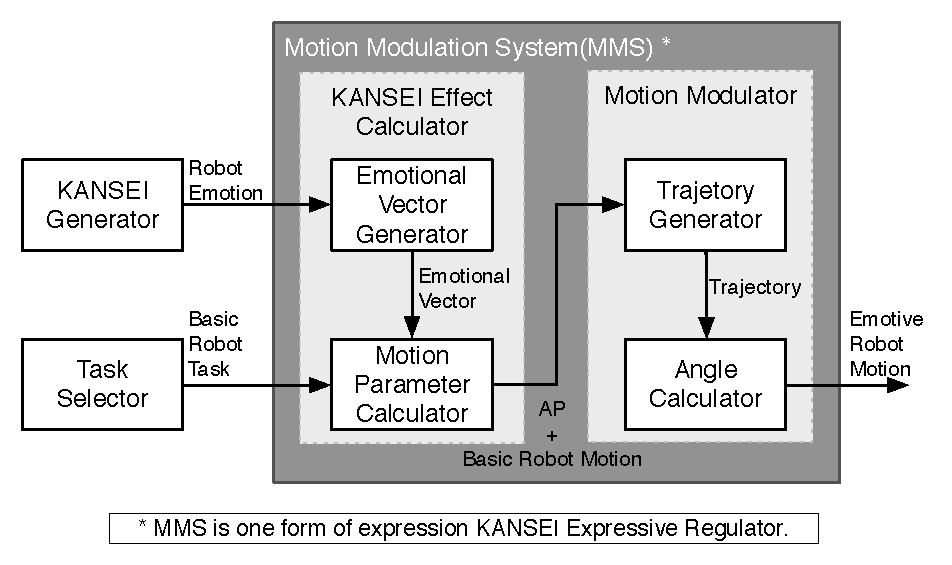
\includegraphics[width=8cm]{MMS.eps}
\vspace{-8mm}
\caption{MMSの内部構成}
\label{fig:mms}
\vspace{2mm}
\end{figure}
\end{verbatim}
}
\end{screen}

\begin{figure}[b]
\centering
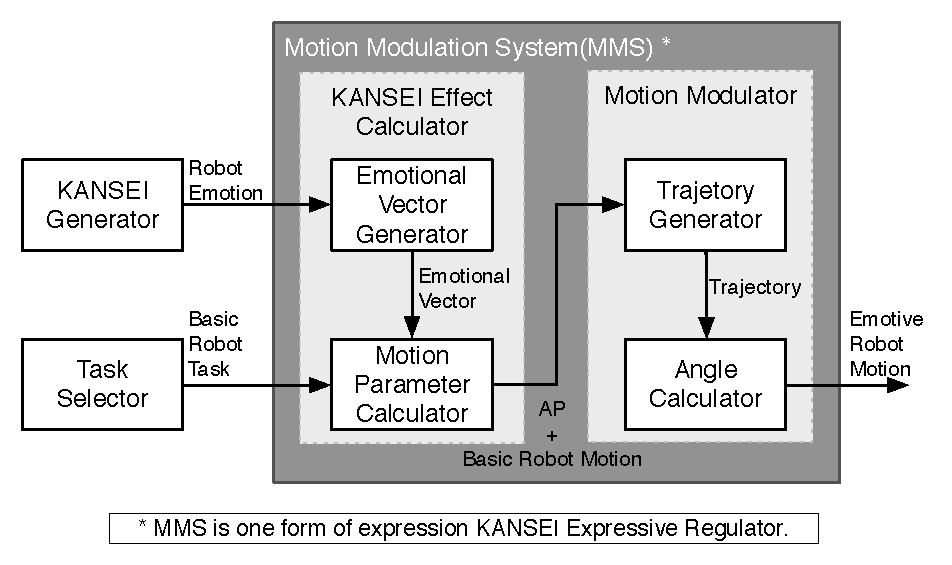
\includegraphics[width=8cm]{MMS.eps}
\vspace{-3mm}
\caption{MMSの内部構成}
\label{fig:mms}
\vspace{5mm}
\end{figure}

